% Trying to break the document up a bit.  This command simply inserts the contents of the file at this point.  It contains the document license, preamble, and title page: things that aren't likely to change more than once.  This can be used to separate discrete parts of a document into files that are easier to edit at one time.
%%%%%%%%%%%%%%%%%%%%%%%%%%%%%%%%%%%%%%%%%%%%%%%%%%%%%%%%%%%%%%%%%%%%%%
% This layout was adapted from one found at latextemplates.com which
% was adapted from another.
%
% License: CC BY-NC-SA 3.0
% (http://creativecommons.org/licenses/by-nc-sa/3.0/)
%
% Original header:
%
% This is a LaTeX version of the sample laboratory report from
% Virginia Tech's copyrighted 08-09 CHEM 1045/1046 lab manual.
% Reproduction of this one appendix section for academic purposes
% should fall under fair use.
%
%%%%%%%%%%%%%%%%%%%%%%%%%%%%%%%%%%%%%%%%%%%%%%%%%%%%%%%%%%%%%%%%%%%%%%

\documentclass{article}

\usepackage{graphicx}
% \usepackage[acronym]{glossaries} % Lets us use acronyms
\usepackage{multicol}
\usepackage{amsmath}
\usepackage{siunitx} % SI units in math mode
\usepackage{subcaption}

\author{}
\title{ELEC-313 \\ Lab 5: CMOS Circuits\\ }
\date{\today}

% \loadglsentries{acronyms} % Actually loads 'acronyms.tex'
% \makeglossaries

\begin{document}

\maketitle

\begin{center}
  \begin{tabular}{lr}
    Date Performed: & October 16, 2013 \\
    Partners:       & Charles Pittman    \\
    & Stephen Wilson     \\
  \end{tabular}
\end{center}

\newpage

\tableofcontents
\listoffigures
\listoftables
\newpage

% Number the enumerate environment (unordered lists) by letter:
\renewcommand{\labelenumi}{\alph{enumi}.}

\section{Objective}

The objective is to construct and observe the operation of a common-emitter transistor amplifier.

\section{Equipment}

\begin{tabular}{ll}
  \centering
  Transistor: 2N2222A & Capacitor: \SI{0.1}{\micro\farad} \\
  Resistors: \SI{100}{\kilo\ohm}, \SI{20}{\kilo\ohm}, \SI{1}{\kilo\ohm}, \SI{470}{\ohm} & Power supply: HP E3631A \\
  Function generator: HP 33120 & Oscilloscope: Agilent 54622D \\
  \multicolumn{2}{l}{Multimeters: HP 34401A, Fluke 8010A (x2)} \\
\end{tabular}

\section{Schematics}

\begin{figure}[hbtp]
  \centering
  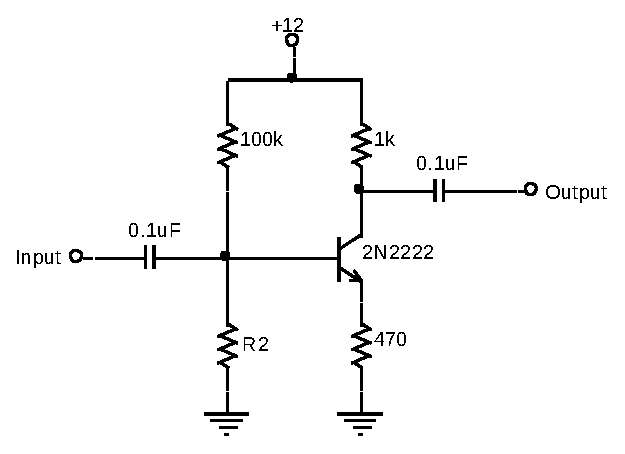
\includegraphics[width=0.7\textwidth]{circuit}
  \caption{\label{fig:circuit} Common-emitter transistor amplifier (without the emitter bypass capacitor). $R_2$ = \SI{20}{\kilo\ohm}}
\end{figure}

\section{Procedure}

\section{Results}

\begin{table}[hbtp]
  \centering
  \begin{tabular}{ccc|cc|c}
    $V_B$    & $V_C$    & $V_E$    & $V_i$     & $V_o$     & $A_V$ \\
    (\si{V}) & (\si{V}) & (\si{V}) & (\si{mV}) & (\si{mV}) &       \\
    \hline
    1.788    & 9.58     & 1.153    & 500       & 970       & 1.94  \\
  \end{tabular}
  \caption{\label{tab:amp} Transistor amplifier characteristics}
\end{table}

\begin{table}[hbtp]
  \centering
  \begin{tabular}{cc}
    $R$         & $V_{OC}$  \\
    (\si{\ohm}) & (\si{mV}) \\
    \hline
    958         & 477       \\
  \end{tabular}
  \caption{\label{tab:imp} Port impedances}
\end{table}

\begin{table}[hbtp]
  \centering
  \begin{tabular}{cc}
    $R$              & $V_i$    \\
    (\si{\kilo\ohm}) & (\si{V}) \\
    \hline
    13.9             & 2.57     \\
  \end{tabular}
  \caption{\label{tab:lrg_sig} Large-signal performance}
\end{table}

\begin{table}[hbtp]
  \centering
  \begin{tabular}{ccc|cc|c}
    $V_B$    & $V_C$    & $V_E$    & $V_i$    & $V_o$    & $A_V$ \\
    (\si{V}) & (\si{V}) & (\si{V}) & (\si{V}) & (\si{V}) &       \\
    \hline
    1.783    & 9.547    & 1.164    & 0.122    & 6.19     & 52.0
  \end{tabular}
  \caption{\label{tab:amp_bypass} Transistor amplifier characteristics (with emitter bypass capacitor)}
\end{table}

%\newpage

\section{Conclusion}
\label{sec:conclusion}

\section{Equations}

% LaTeX sees blank lines as a start of another paragraph.  To avoid
% unnecessary vertical spaces between equations, and still visually
% separate in source, put a comment between them.
%
% \begin{equation}
%   \label{eq:beta}
%   \beta = \frac{I_C}{I_B}
% \end{equation}
% %
% \begin{equation}
%   \label{eq:hoe}
%   h_{oe} \approx \frac{1}{r_o} = \frac{\Delta I_C}{\Delta V_{CE}}
% \end{equation}
%
% \begin{equation}
%   \label{eqn:percent_diff}
%   \%_{diff} = \frac{|measured - theoretical|}{theoretical} \times 100\%
% \end{equation}

\end{document}
